\chapter{Grundlagen}
\label{cha:basics}

In diesem Kapitel wird zunächst auf die Motivation für ein \gls{SoC} und dessen Grundaufbau eingegangen. In diesem Zusammenhang wird auf die Bus-Architekturen \enquote{Wishbone} und \enquote{Avalon} eingegangen. Danach wird das Plasma-System von Steve Rhoads, sowie die Entwicklungs- und Evaluationsboards ZedBoard \cite{manual:zedboard} von Digilent und DE1-SoC \cite{manual:de1soc} von Terasic vorgestellt.

\section{System-On-Chip}

Der Begriff \gls{SoC} wurde durch die Integration eines gesamten Systems (Prozessor, Speicher und Peripherie) auf einem einzigen Chip geprägt.
Die \glspl{SoC} sind aus modernen Geräten nicht wegzudenken. Ein prägnantes Beispiel hierfür ist ein Smartphone: auf einem einzigen Chip sind beispielsweise eine \gls{CPU}, \gls{GPU}, \gls{GSM}-Modem, ein Display-Controller sowie der Kamera-Controller samt einem \gls{DSP} zur Bildverarbeitung integriert. Moderne Medizin-, Automobil-, Avionik-, Raumfahrt- und Militär-Systeme wären ohne \glspl{SoC} nicht möglich. Doch auch banal erscheinende Geräte wie Küchengeräte und sogar die Heimbeleuchtung (\gls{IoT} und Smart-Home) profitieren von der zunehmenden Miniaturisierung und den Einsatzmöglichkeiten der \glspl{SoC}. 

Der Entwurf eines \gls{SoC} ist mit einem sehr hohen Zeit- und Arbeitsaufwand verbunden. Je komplexer das System, desto aufwändiger wird ein von Grund auf neuer Aufbau. \cite[189]{book:embedded_sopc_design} Darum wird heutzutage, analog zur Softwareentwicklung, auf erprobte, wiederverwendbare Komponenten gesetzt. Diese sind als IP-Cores verfügbar und können in eigene Projekte integriert werden. Davon sind einige parametrisierbar und somit auf Projektbedürfnisse anpassbar. Ein IP-Core kann als high-level \gls{HDL} Code, auch Soft-Core genannt, oder auch als ein detailliertes Layout auf Transistorebene, Hard-Core genannt, ausgeliefert werden. \cite[189]{book:embedded_sopc_design} 

Ein gutes Beispiel für parametrisierbare IP-Cores ist die \gls{ARM}-CPU. ARM als Unternehmen ist kein Prozessorhersteller an sich, sondern bietet ledeglich die \gls{CPU}-Architektur als IP-Core zur Erwerb an. Ein Interessent kann diese lizenzieren, auf seine Bedürfnisse anpassen und bei einem Halbleiterfertiger in Produktion geben. Durch Kombination verschiedener auf dem Markt verfügbarer IP-Cores kann innerhalb kürzester Zeit ein neues Produkt mit einem gegenüber den Einzelkomponenten erhöhten Mehrwert entwickelt werden.

\section{Bussysteme}
\label{the:bus_system}
In vorigen Abschnitten wurden beispielhaft einige Komponenten eines \gls{SoC} genannt. Im Wesentlichen handelt es sich hierbei um eine \gls{CPU}, die mit sämtlichen domänenspezifischen Prozessoren und Peripheriegeräten bzw. Schnittstellen kommuniziert. Essentiell hierfür ist ein Bus-System, welches allen relevanten Modulen ein Kommunikationsmedium bereitstellt. Verbreitet sind standardisierte Bus-Architekturen wie AMBA, CoreConnect, Wishbone, STBus und weitere. \cite[2]{article:soc_buses} AMBA ist sehr verbreitet in der Entwicklung von \glspl{SoC} auf Basis von \gls{ARM}-Prozessoren. In dieser Arbeit wird besondere Aufmerksamkeit dem Wishbone- und Avalon-Bus gewidmet. 

\subsection{Topologien}

Unter einer Bus-Topologie versteht man die Anordnung der Master- und Slavegeräte zueinander. Je nach Topologie muss u.U. eine Arbitrierung vorgenommen werden, um Ressourcen unter mehreren Teilnehmern verteilen zu können. Die nachfolgenden Abbildungen entstammen der Wishbone-Spezifikation \cite{website:wishbone_b4_spec} und sind auch auf andere Bussysteme übertragbar. 

\begin{figure}[!htbp]
	\centering
	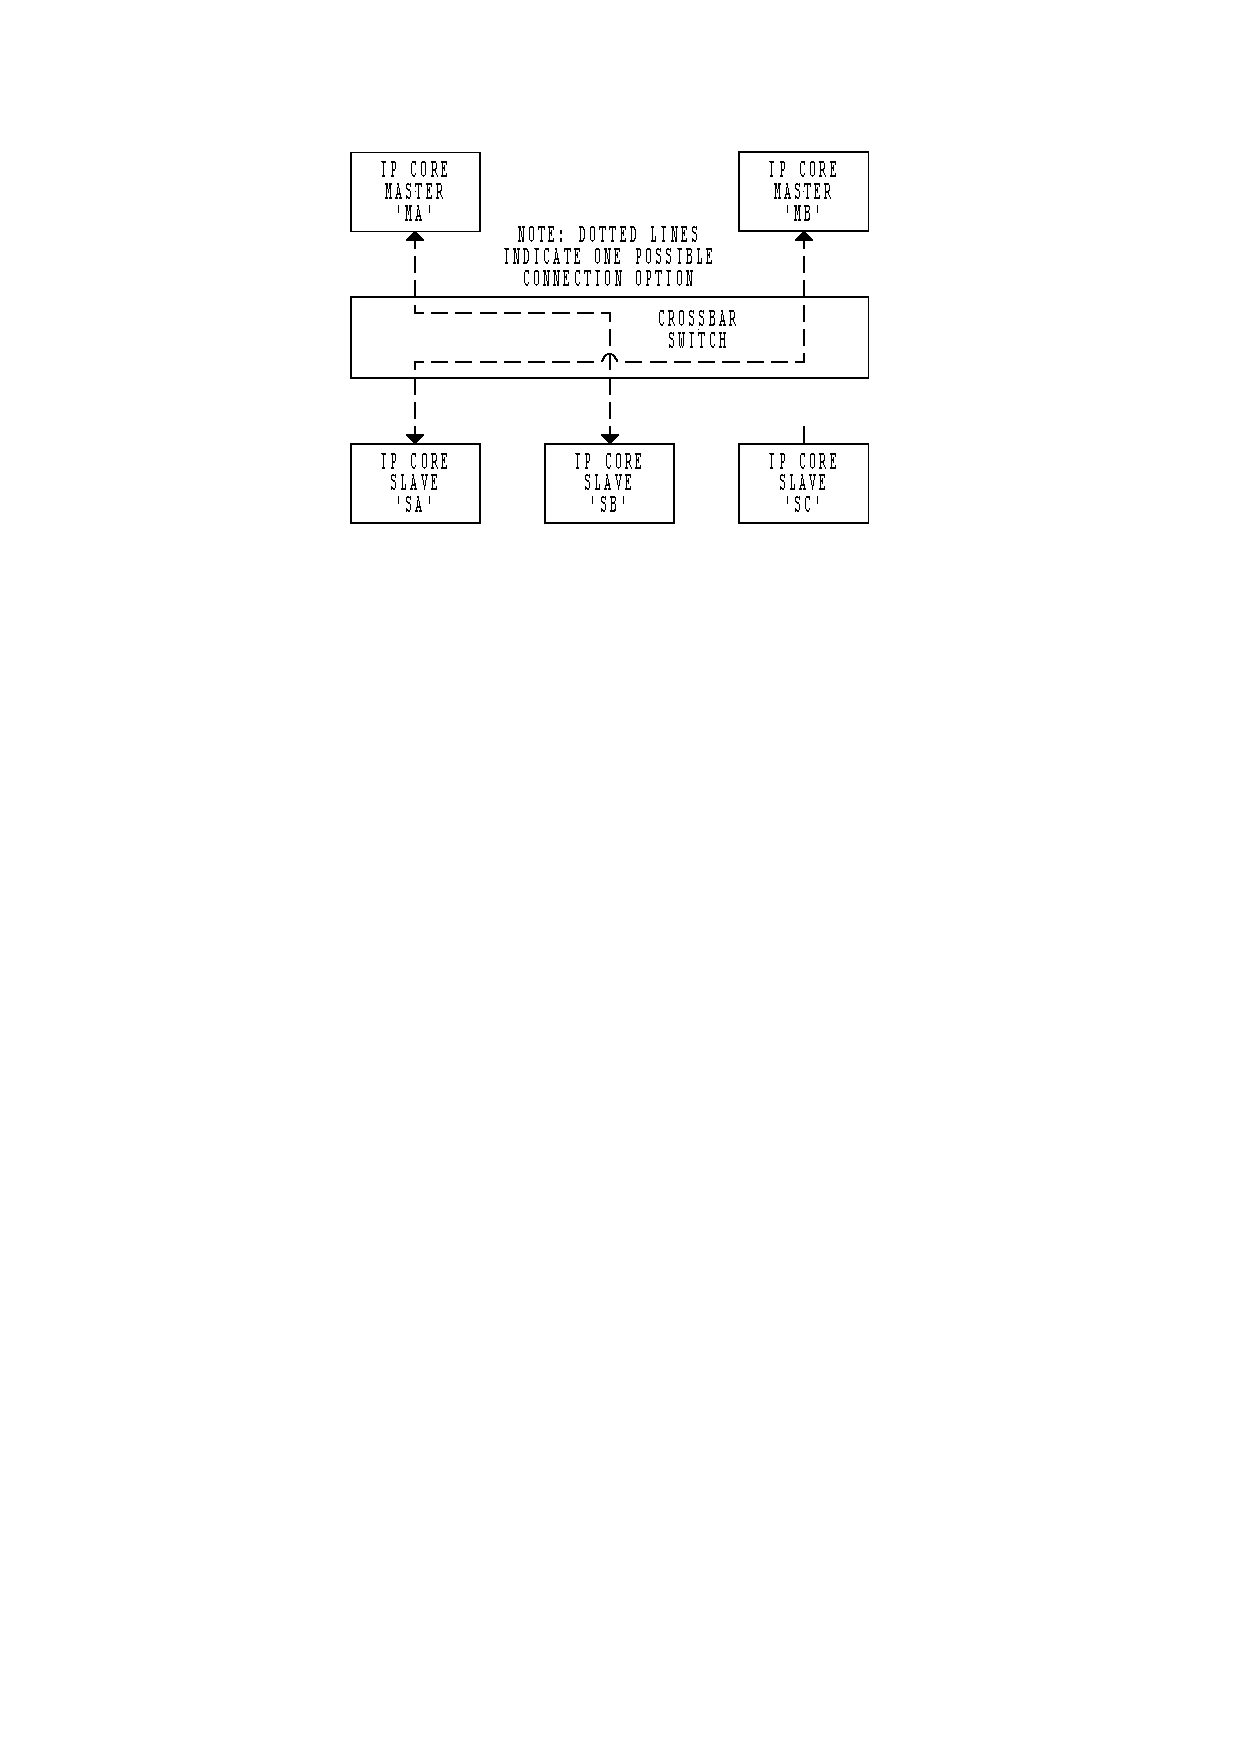
\includegraphics[width=0.6\linewidth]{images/crossbar_switch_interconnection}
	\caption{Crossbar (Switch) \cite[17]{website:wishbone_b4_spec}}
	\label{fig:crossbar_switch_intercon}
\end{figure}

In \cref{fig:crossbar_switch_intercon} ist eine Crossbar-Switch-Topologie dargestellt. In diesem Fall können mehrere Master zeitgleich eine Verbindung zu einem Slave aufnehmen. Jede Verbindung ist unabhängiig von den anderen und kann parallel betrieben werden. Durch diese Parallelität erhöht sich der Durchsatz des ganzen Systems. Diese Topologie ist geschwindigkeitsmäßig den klassischen Bussystemen überlegen. Grundsätzlich unterstützen die Crossbar Routingmechanismen dynamische Konfiguration, was zu einen zuverlässigem und konfigurierbaren Netzwerk führt. Außerdem sind die meisten Crossbar-Architekturen skalierbar, können also bei Bedarf erweitert werden. \cite[16]{website:wishbone_b4_spec}

\begin{figure}[!htbp]
	\centering
	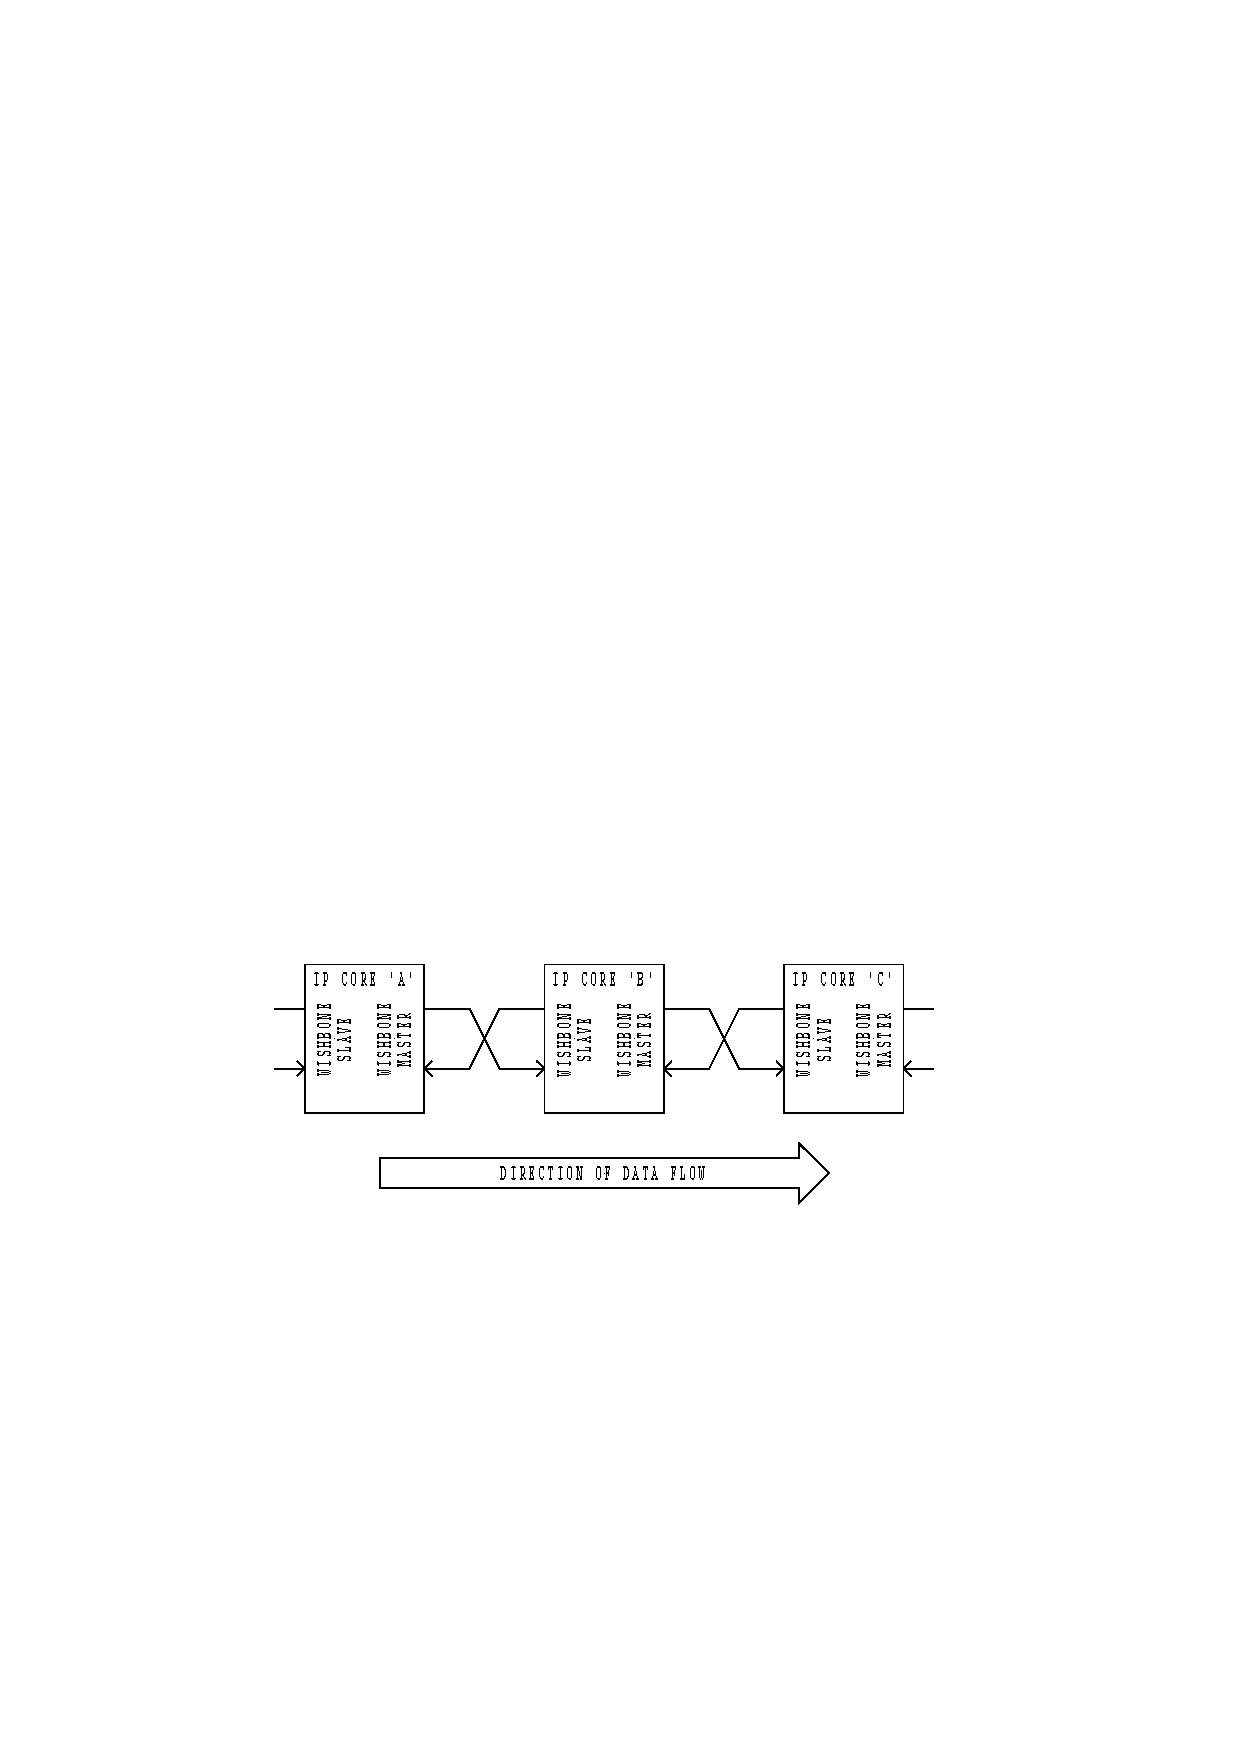
\includegraphics[width=0.9\linewidth]{images/data_flow_interconnection}
	\caption{Data flow \cite[17]{website:wishbone_b4_spec}}
	\label{fig:data_flow_intercon}
\end{figure}

In \cref{fig:data_flow_intercon} ist eine Data-Flow-Topologie dargestellt. Hierbei fließt der Datenstrom sequentiell durch einen vordefinierten Satz an IP-Cores. Data-Flow-Architekturen weisen oft eine Parallelität auf: eine oder mehrere werden Funktionen zeitgleich ausgeführt. \cite[17]{website:wishbone_b4_spec}

\begin{figure}[!htbp]
	\centering
	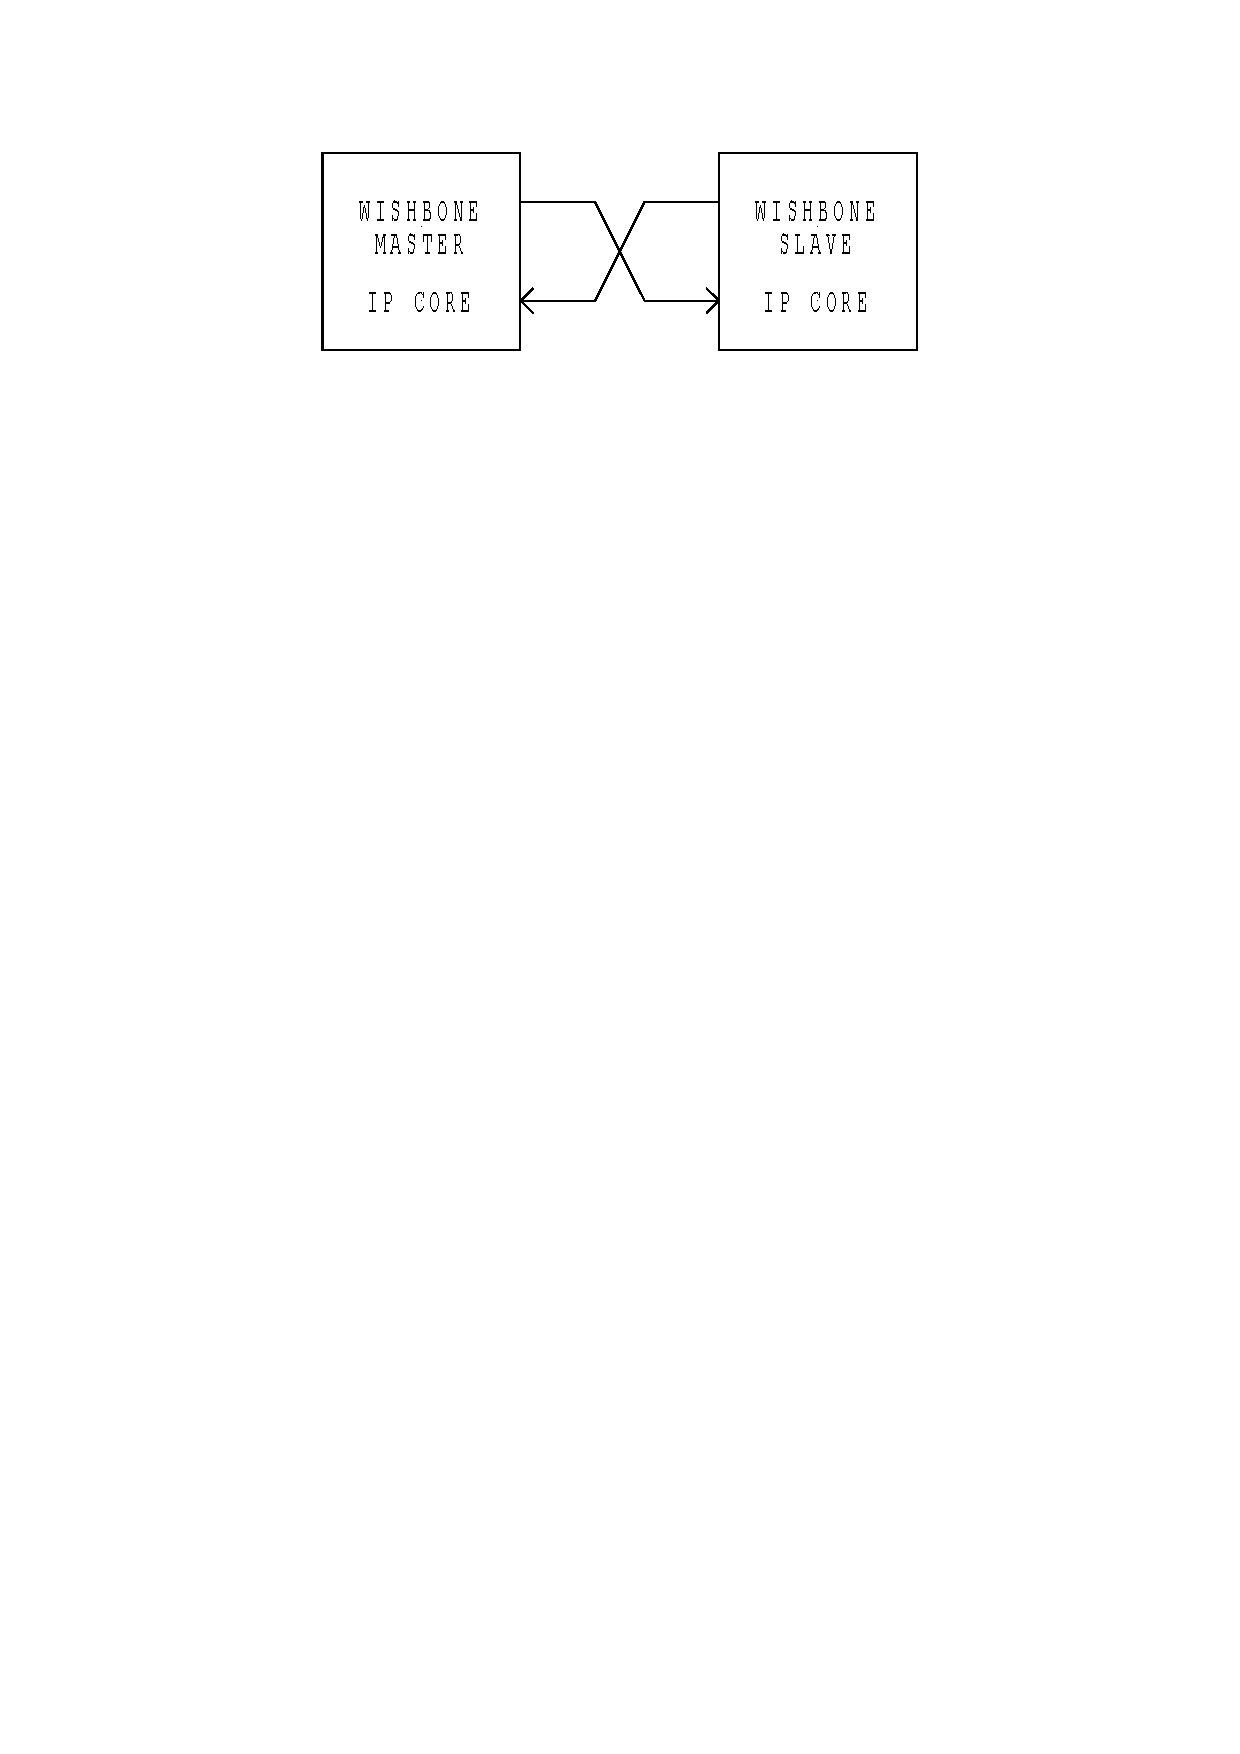
\includegraphics[width=0.6\linewidth]{images/point_to_point_interconnection}
	\caption{Point to point \cite[21]{website:wishbone_b4_spec}}
	\label{fig:p2p_intercon}
\end{figure}

Eine Punkt-zu-Punkt Topologie, wie in \cref{fig:p2p_intercon} abgebildet, ist die einfachste aller Topologien mit einem einzigen Master und einem Slave.\cite[20]{website:wishbone_b4_spec}

\begin{figure}[!htbp]
	\centering
	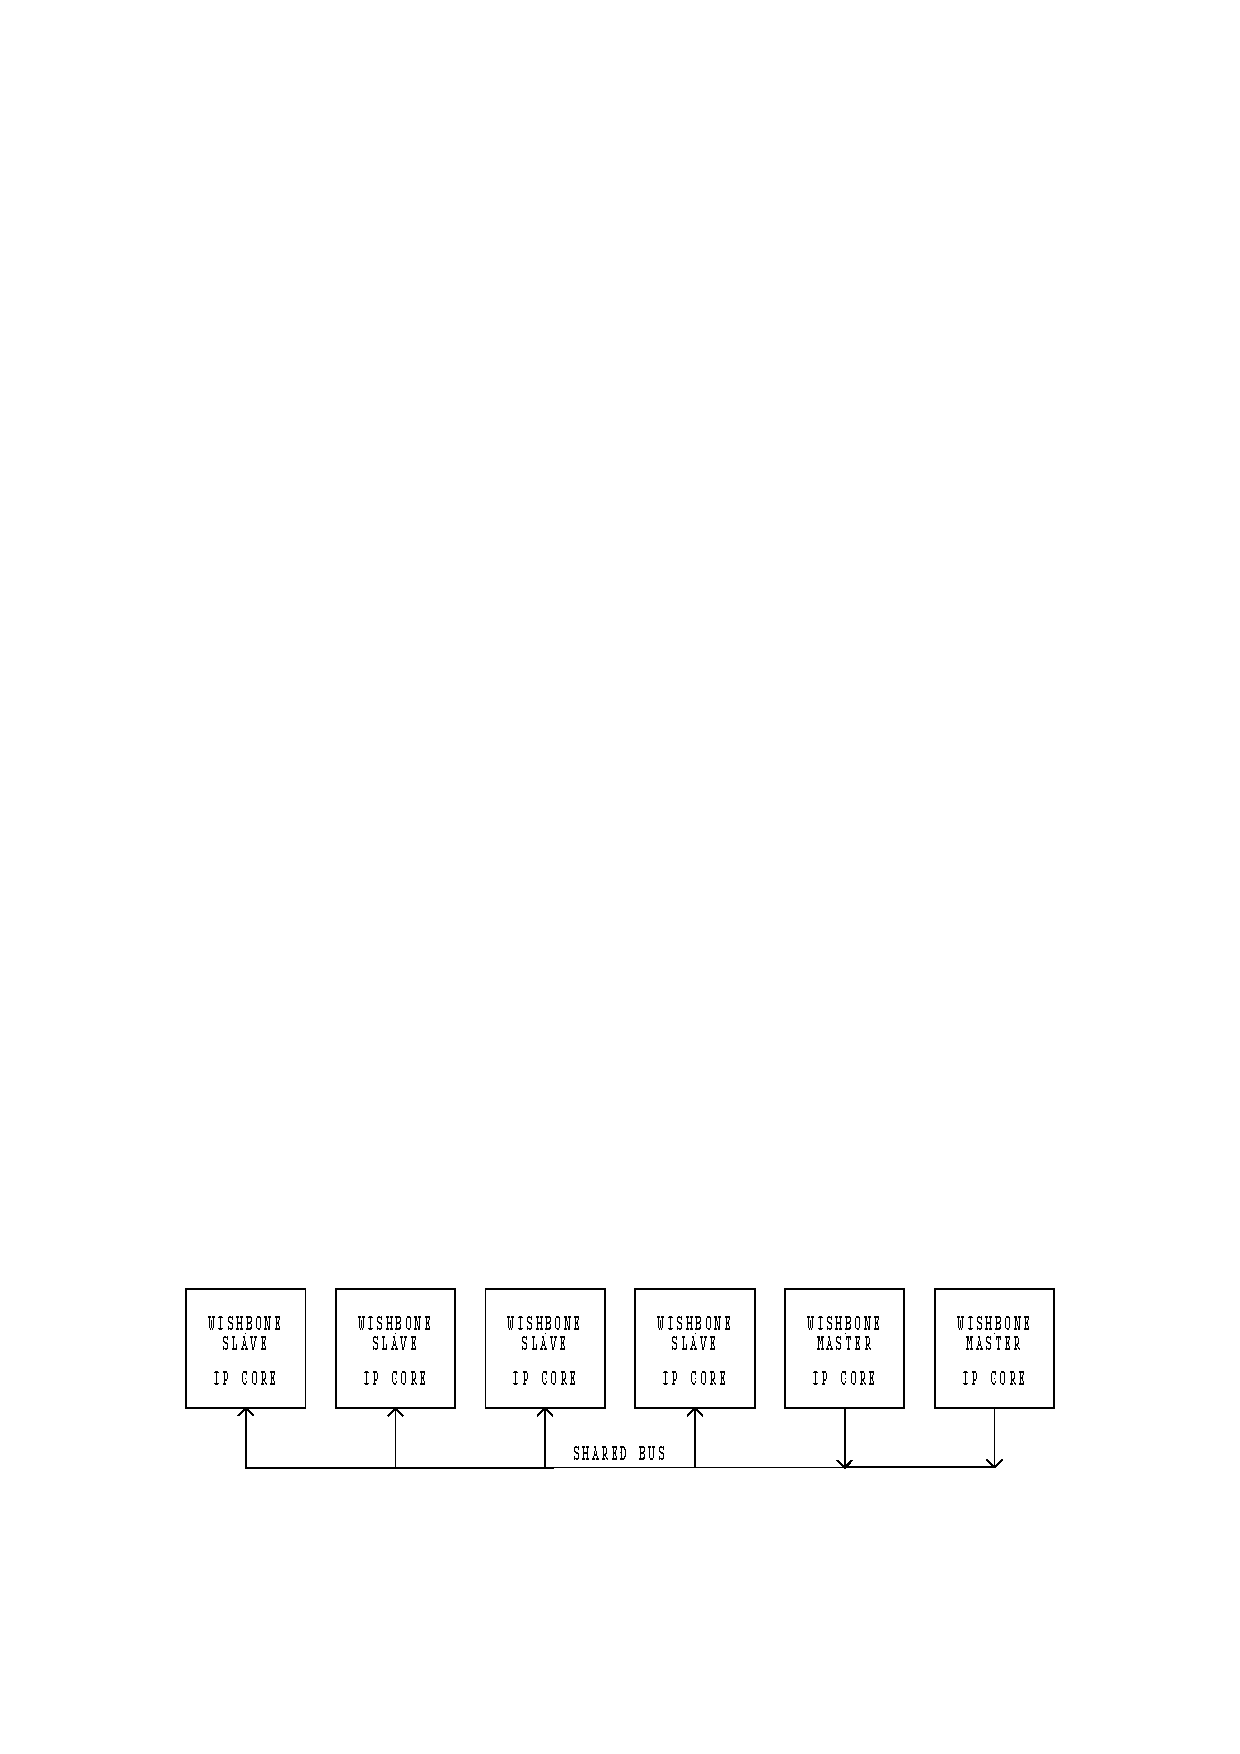
\includegraphics[width=0.9\linewidth]{images/shared_bus_interconnection}
	\caption{Shared bus \cites[21]{website:wishbone_b4_spec}}
	\label{fig:shared_bus_intercon}
\end{figure}

In \cref{fig:shared_bus_intercon} ist eine Shared-Bus-Topologie dargestellt. Hierbei initiiert ein Master einen Buszyklus zum Slave. Traditionelle Busse wie VMEbus und PCI Bus nutzen diese Topologie. Architekturbedingt kann hier nur ein Master zu einem Zeitpunkt den Bus nutzen. \cite[21]{website:wishbone_b4_spec}

\subsection{Wishbone}

Wishbone ist ein Open-Source-Hardware Computerbus, welcher die Kommunikation der Komponenten eines \gls{SoC} durch eine einheitliche Schnittstelle deutlich vereinfacht. Entwickelt wurde dieser von der Silicore Corporation, und später von OpenCores\footnote{\url{https://opencores.org}} veröffentlicht. Überwiegend wird Wishbone-Standard von quelloffenen Hardware-Projekten verwendet. 

Eine mögliche Portkonfiguration für Wishbone-Master bzw Slave ist in \cref{fig:standard_connection_for_timing_diagrams} dargestellt.

\begin{figure}[!htbp]
	\centering
	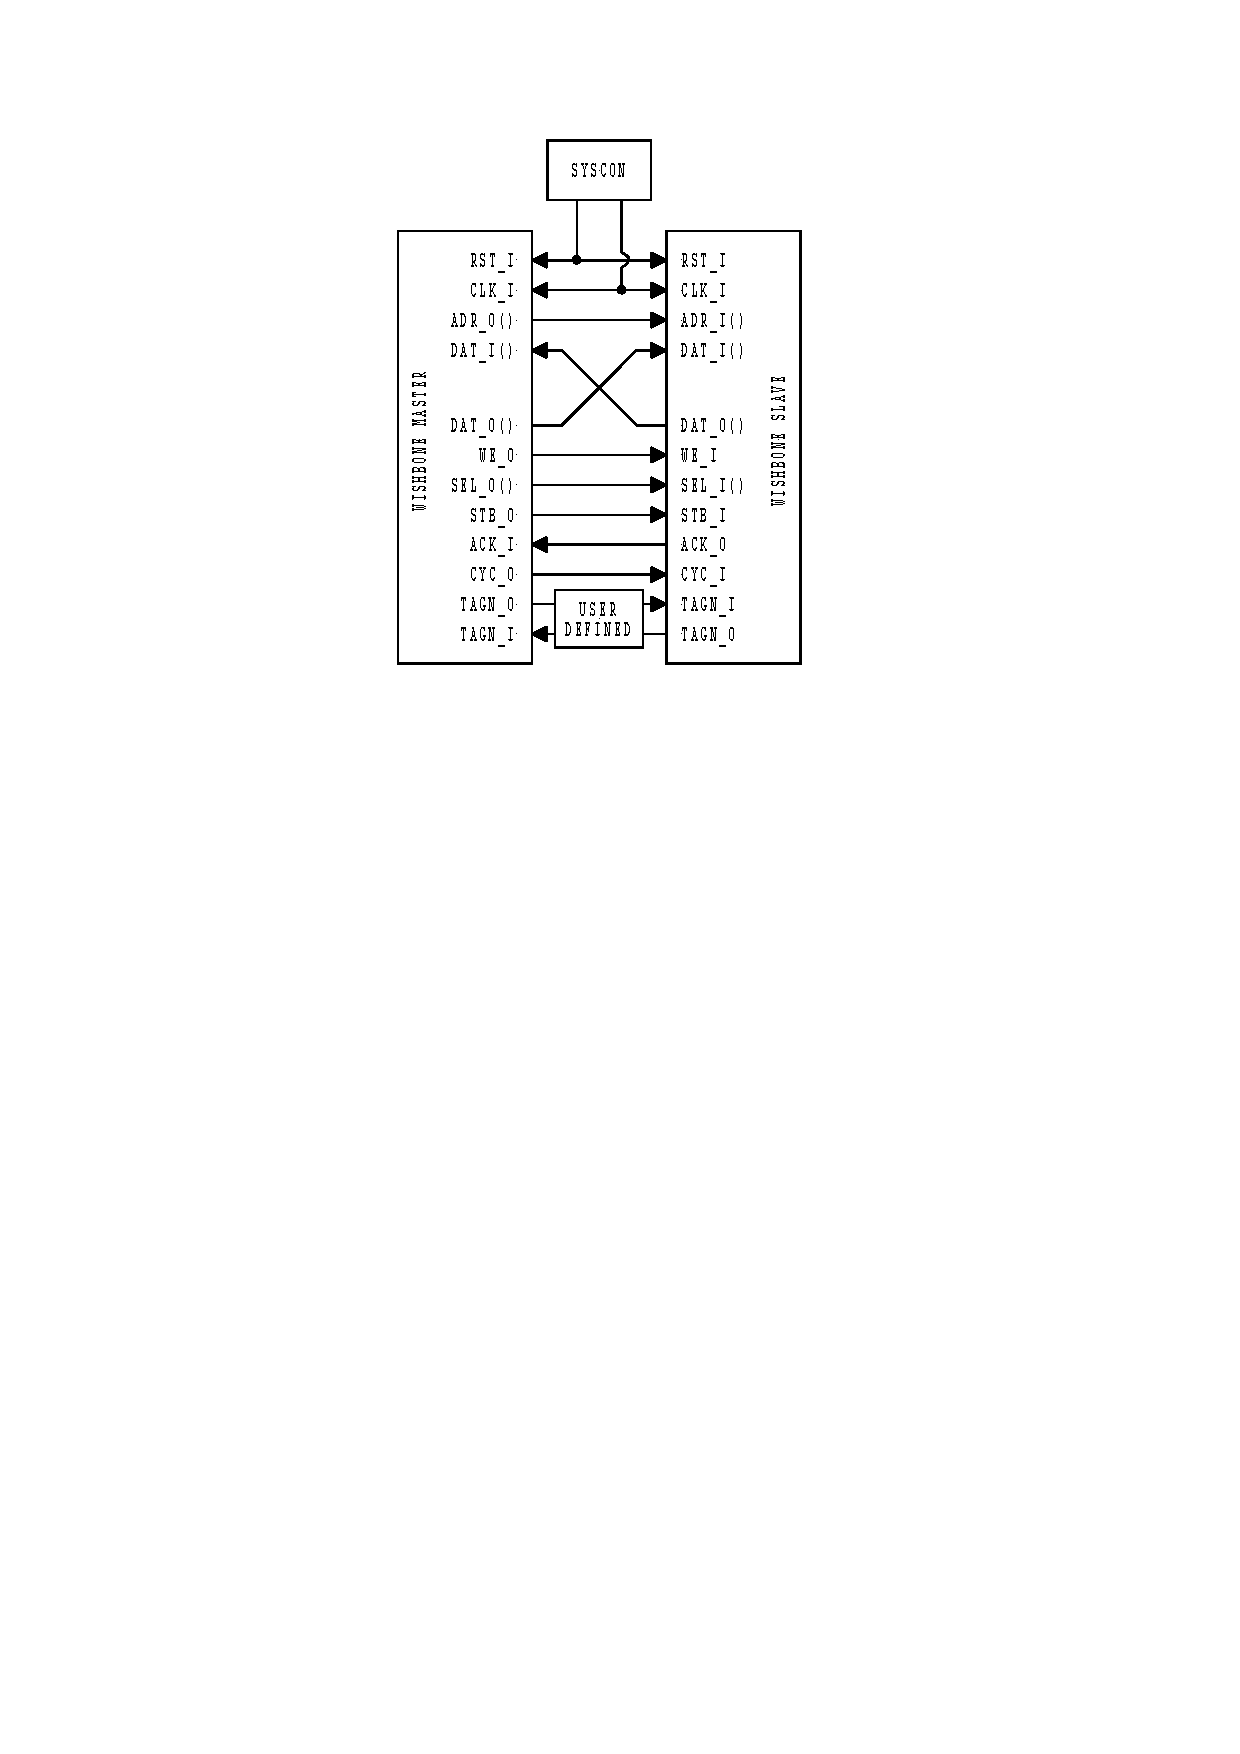
\includegraphics[width=0.5\linewidth]{images/standard_connection_for_timing_diagrams}
	\caption{Standard connection for timing diagrams \cite[14]{website:wishbone_b4_spec}}
	\label{fig:standard_connection_for_timing_diagrams}
\end{figure}

\subsection{Avalon}
\label{sec:theory_avalon}

Avalon ist eine proprietäre Bus-Architektur und wurde ursprünglich von Altera entwickelt, um On-Chip-Prozessoren und Peripherie zu einem \gls{SOPC} zu verknüpfen. \cite[{7-6}]{article:soc_buses} Nutzbar ist Avalon als eine Sammlung parametrisierbarer IP-Cores, die vom Platform Designer (früher als Qsys bzw. SOPC Builder bekannt) im Laufe der Systementwicklung automatisch generiert und parametrisert werden. 

Ein mögliches System mit Avalon ist auf \cref{fig:avalon_bus_based_system} abgebildet.

\begin{figure}[!htbp]
	\centering
	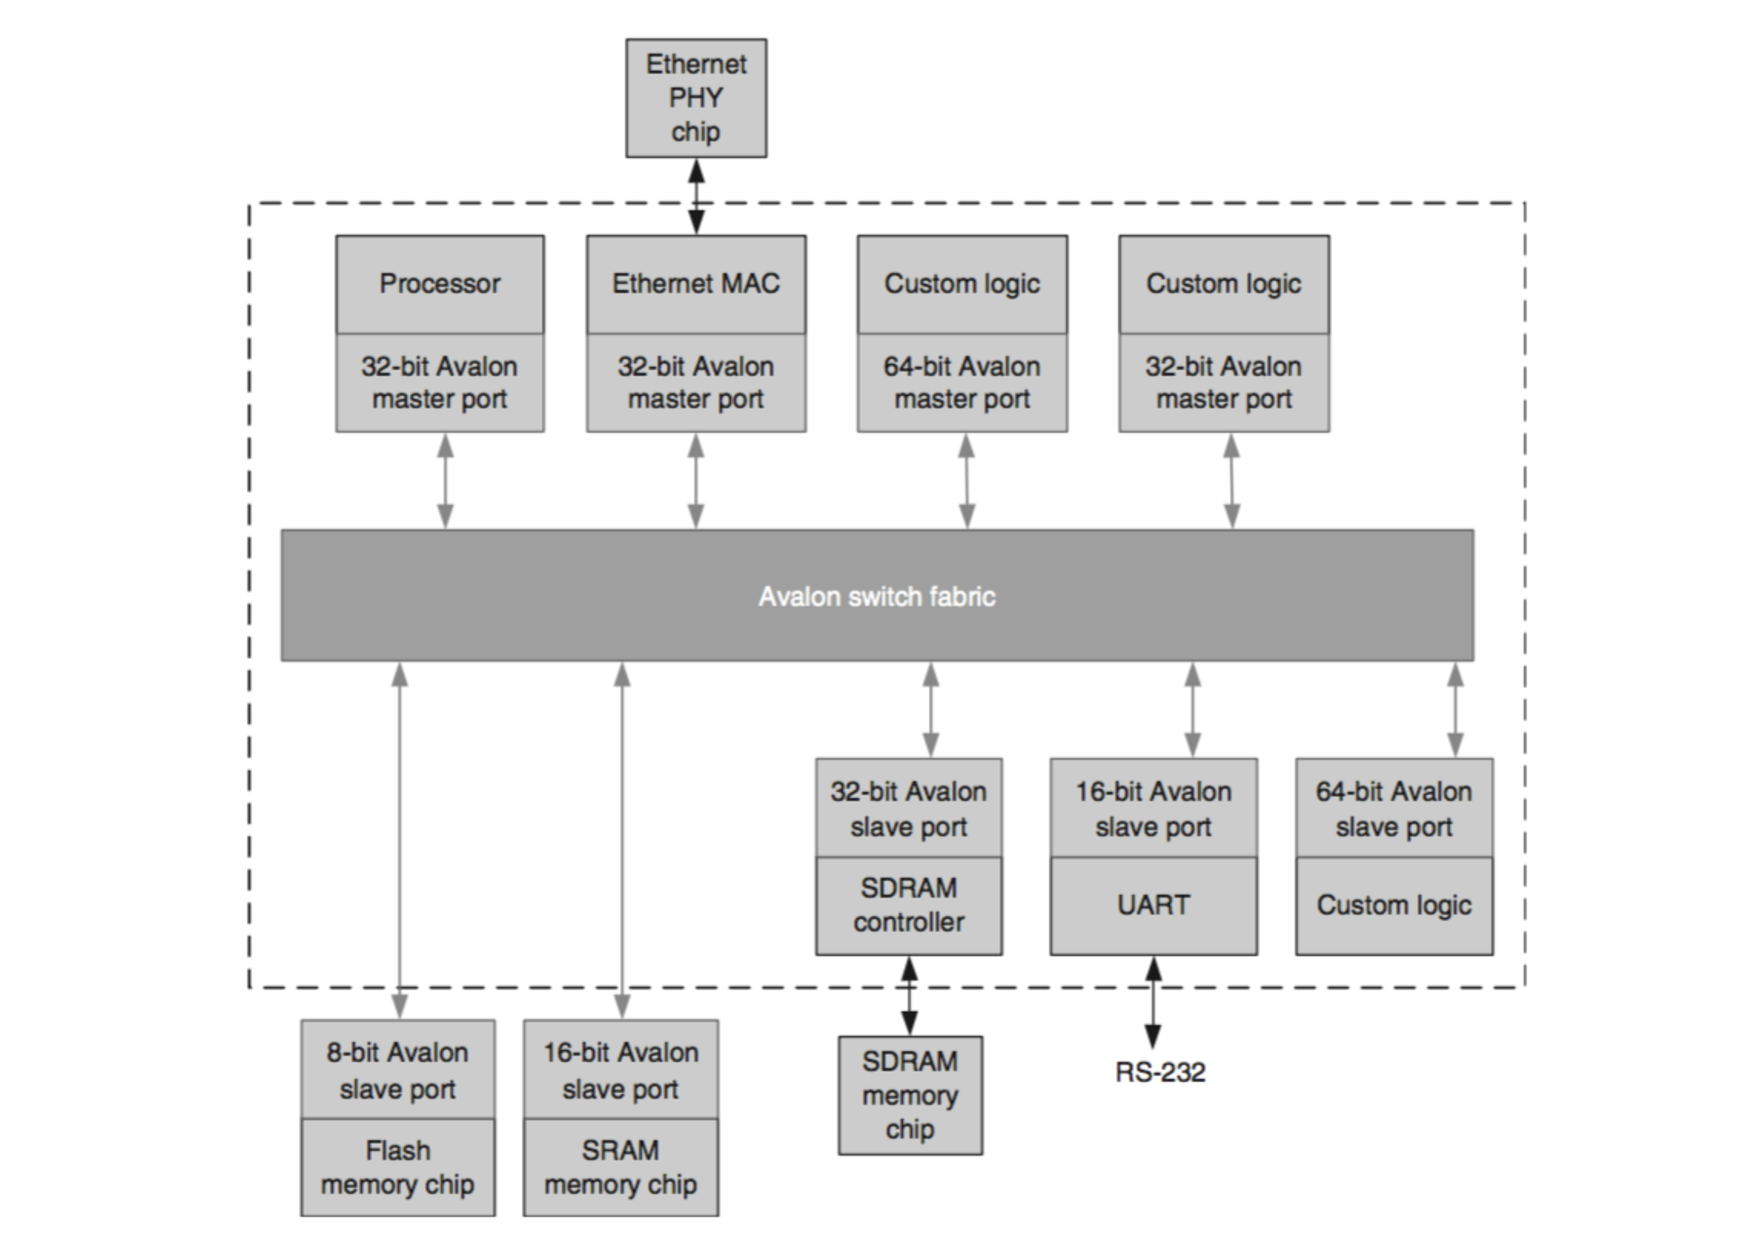
\includegraphics[width=0.7\linewidth]{images/avalon_bus_based_system}
	\caption{Avalon-Bus basiertes System \cite[{7-6}]{article:soc_buses}}
	\label{fig:avalon_bus_based_system}
\end{figure}

Die Avalon-Spezifikation sieht sieben Schnittstellentypen vor \cite[4]{manual:avalon_spec}: 
\begin{easylist}[itemize]
	& Avalon Streaming Interface (Avalon-ST) - unterstützt unidirektionalen Datenfluss (vgl. \cref{fig:data_flow_intercon})
	& Avalon Memory Mapped Interface (Avalon-MM) - unterstützt adressbasierte bidiriektionale Master-Slave Kommunikation 
	& Avalon Conduit Interface - fasst Signale, die nicht einem Avalon-Schnittstellentyp zuzuordnen sind, zusammen. Eine Verbindung im Platform Designer bzw. Export zur manuellen Verknüpfung ist möglich
	& Avalon Tri-State Conduit Interface (Avalon-TC) - unterstützt Verbindungen zu Off-Chip Komponenten. Mehrere Peripheriegeräte können Pins durch Signalmultiplexing teilen
	& Avalon Interrupt Interface - ermöglicht Komponenten Ereignisse an andere Komponenten zu vermitteln
	& Avalon Clock Interface - Schnittstelle für Taktein- bzw. Ausgang
	& Avalon Reset Interface - Schnittstelle für Reset-Logik	
\end{easylist}

Avalon nutzt separate Adress-, Daten-, und Steuerleitungen. \cite[7-6]{article:soc_buses}
In \cref{tab:avalonmm_signals} sind die für diese Arbeit wichtigsten Avalon-MM Signale aufgelistet.
\begin{table}[!htbp]
	\bigskip
	\centering
	\begin{tabular}{  l | l }
		\textbf{Signal} & \textbf{Beschreibung} \\
		\hline
		address & Adresse \\
		byteenable & Byte-Selektor \\		
		read & Signalisiert einen Lesezugriff \\ 
		write & Signalisiert einen Schreibzugriff \\ 
		readdata & Vom Slave übertragenes Datenwort \\
		writedata & An den Slave übertragenes Datenwort \\
		waitrequest & An den Master übermitteltes Wartesignal \\
		response & Optionaler Antwortcode \\
		\hline
	\end{tabular}
	
	\caption{Avalon-MM Signale \cite[14-16]{manual:avalon_spec}}
	\label{tab:avalonmm_signals}
\end{table}

\section{Plasma CPU}
\label{the:plasma}

Die Plasma \gls{CPU} ist ein kleiner, synthetisierbarer 32-bit \gls{RISC} Mikroprozessor. Derzeit führt es einen Webserver mit einem Interruptcontroller, \gls{UART}, \gls{SRAM} oder \gls{DDR SDRAM} Controller, und einem Ethernetcontroller aus. Die Plasma CPU führt bis auf unausgerichtete Lade und Speicheroperationen alle \gls{MIPS} \RN{1} User-Mode Instruktionen aus \cite{website:plasma_cpu}.

Der auf dem Plasma ausgeführte Webserver ist unter der angegebenen Adresse \textit{https://plasmacpu.no-ip.org:8080/} \cite{website:plasma_cpu}, geprüft am \DTMdate{2018-04-22}, nicht erreichbar.

In \cref{fig:plasma_cpu_block_diagram} ist das Block-Diagramm der Plasma-\gls{CPU} dargestellt.

\begin{figure}[!htbp]
	\centering
	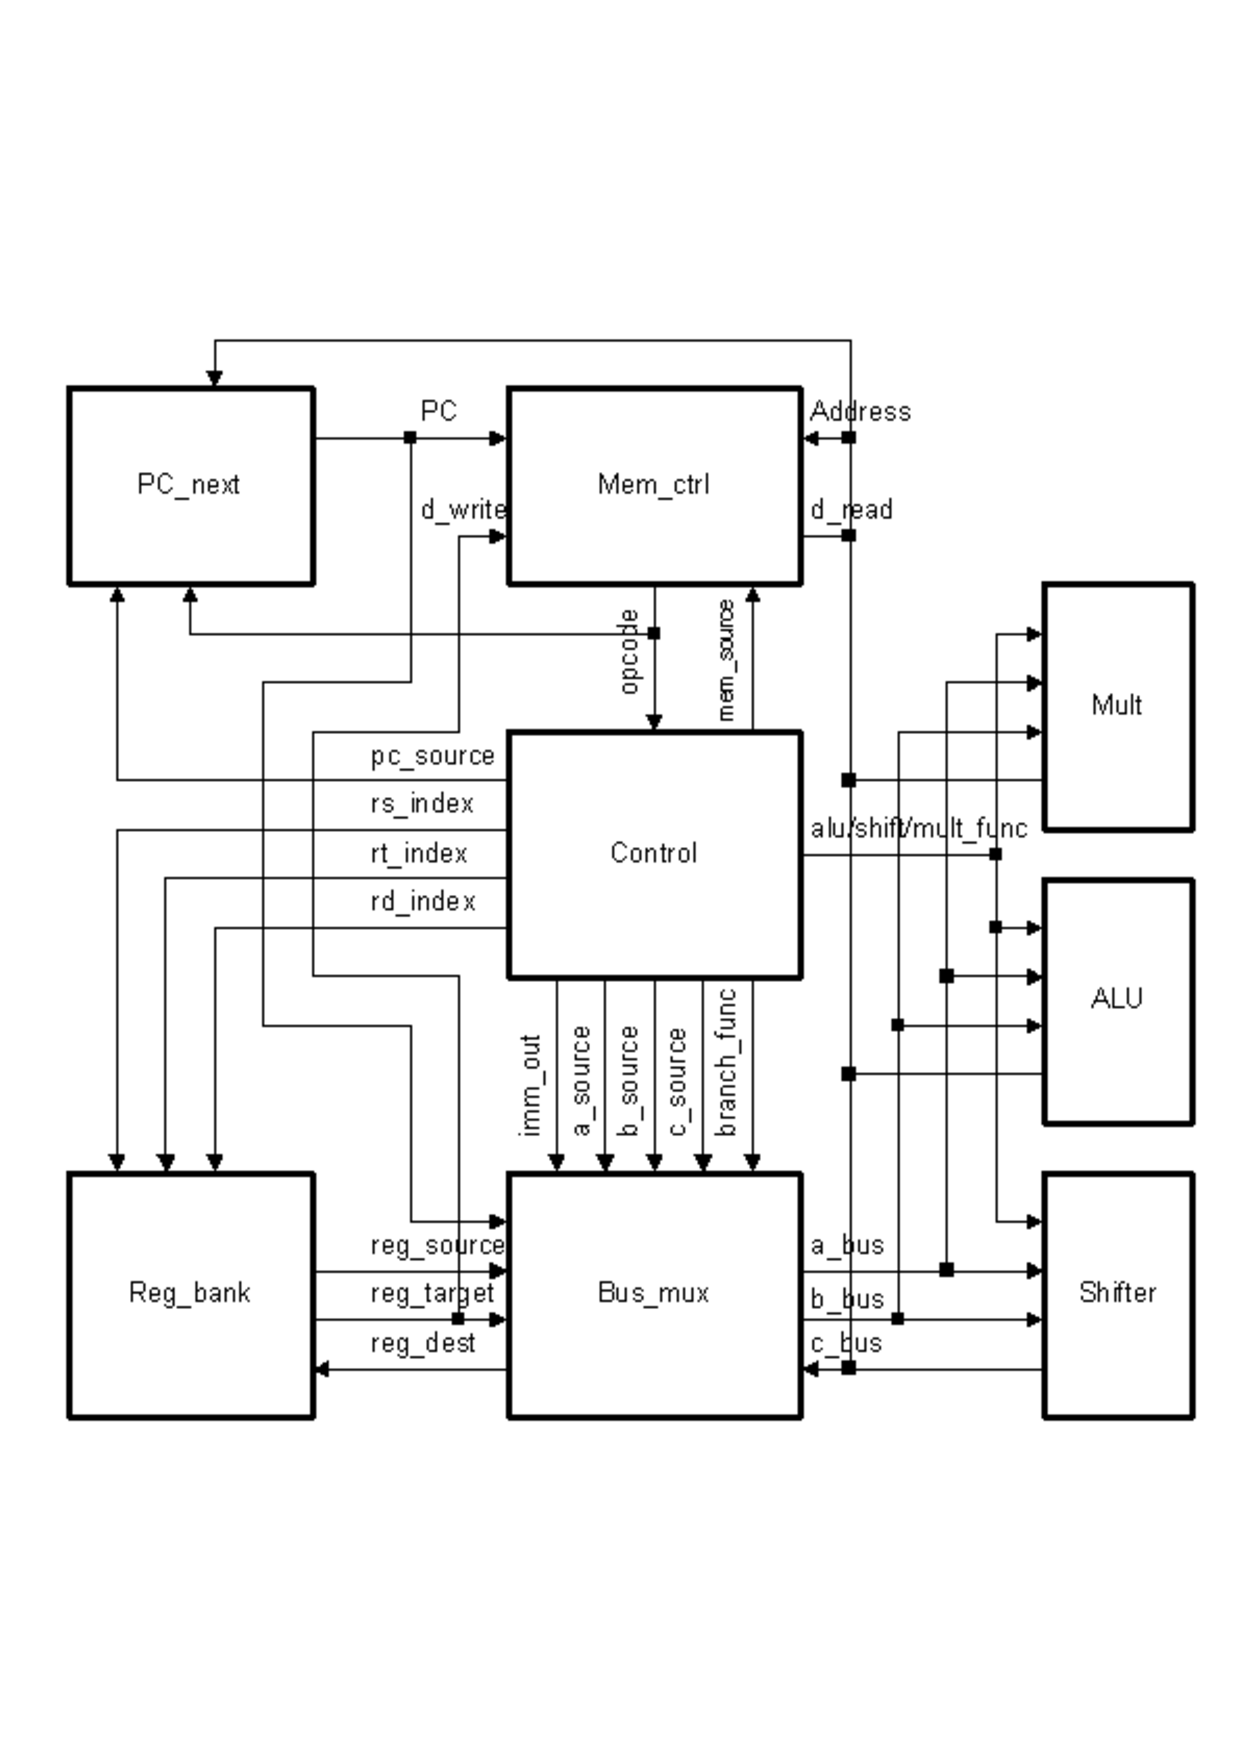
\includegraphics[width=0.6\linewidth]{images/plasma_block_diagram}
	\caption{Plasma-CPU Blockdiagramm \cite{website:plasma_cpu}}
	\label{fig:plasma_cpu_block_diagram}
\end{figure}



\section{Device Tree}

Der Device Tree ist eine baumartige Datenstruktur, mit der eine deklarative Beschreibung der auf einem System verfügbaren Hardware  möglich ist. Jeder Knoten hat Schlüssel/Wert-Paare, welche die Charakteristika des repräsentierten Geräts beschreiben. Die Baum-Struktur ist dadurch gegeben, dass jeder Knoten genau einen Elternknoten besitzt. Die einzige Ausnahme ist der Wurzelknoten, welcher keinem Elternknoten zugeordnet ist \cite[6]{manual:devicetree_specification}. 

Bevor die Device Tree-Spezifikation eingeführt wurde, beinhaltete der Linux-Kernel gerätespezifischen Code. Bereits geringfügige Änderungen, wie die Änderung einer Basisadresse, führten dazu, dass der ganze Kernel neu kompiliert werden musste \cite[1]{manual:intro_to_devicetrees}. 

Für eingebettete Systeme, welche im Gegensatz zu größeren Systemen wie Desktop-Computern nur selten über automatische Erkennungsmechanismen neuer Hardware verfügen, bedeutet es einen enormen Entwicklungs- und Wartungsaufwand. Dieser Aufwand übertrug sich auch auf die Kernel-Entwickler, die Unmengen an verschiedensten Systemkonfigurationen im Kernel verwalten mussten.  

%In \cref{lst:dts_gpio_expl} ist eine beispielhafte Definition für ein \gls{GPIO}-Device dargestellt. Diese wird schrittweise näher erklärt. 
%\begin{code}
%	\begin{minted}[breaklines, autogobble]{text}
%	gpio0: gpio@ff708000 {
%		#address-cells = <1>;
%		#size-cells = <0>;
%		compatible = "snps,dw-apb-gpio";
%		reg = <0xff708000 0x1000>;
%		clocks = <&l4_mp_clk>;
%		status = "disabled";
%		
%		porta: gpio-controller@0 {
%			compatible = "snps,dw-apb-gpio-port";
%			gpio-controller;
%			#gpio-cells = <2>;
%			snps,nr-gpios = <29>;
%			reg = <0>;
%			interrupt-controller;
%			#interrupt-cells = <2>;
%			interrupts = <0 164 4>;
%		};
%	};
%	\end{minted}
%	
%	\caption{Devicetree: Komponenten am Avalon-Bus}
%	\label{lst:dts_gpio_expl}
%\end{code}
%
%
%Der Ausdruck \texttt{gpio0} definiert das Label, wodurch die nachfolgende Gerätebeschreibung an anderen Stellen referenziert werden kann. Der Ausdruck \texttt{gpio} definiert den Gerätetypen und \texttt{ff708000} die Basisadresse:
%\begin{minted}[breaklines, autogobble]{text}
%	gpio0: gpio@ff708000
%\end{minted}
%
%Das Rautenzeichen (\#) gibt an, dass der Schlüssel einen \SI{32}{\bit} breiten vorzeichenlosen Ganzzahlwert annimmt.
%Mit \texttt{address-cells} und \texttt{size-cells} wird die Adressierungsart der Kinderknoten spezifiziert. In diesem Beispiel werden \SI{32}{\bit} (eine Zelle) für die Adresskodierung und \SI{0}{\bit} (0 Zellen) für den Adressbereich genutzt:
%\begin{minted}[breaklines, autogobble]{text}
%#address-cells = <1>;
%#size-cells = <0>;
%\end{minted}
%
%Der Schlüssel \texttt{compatible} gibt den kompatiblen Treiber an. Wenn dieser vorhanden ist, so wird er vom Kernel geladen und an diese Gerätebeschreibung gebunden:
%\begin{minted}[breaklines, autogobble]{text}
%compatible = "snps,dw-apb-gpio";
%\end{minted}
%
%Mit dem \texttt{reg}-Schlüssel wird nochmals die Basisadresse angegeben. Hinzu kommt der Adressbereich \texttt{0x1000}:
%\begin{minted}[breaklines, autogobble]{text}
%reg = <0xff708000 0x1000>;
%\end{minted}
%
%Der \texttt{clocks}-Schlüssel gibt die Taktgeber an. Hierbei wird auch der Einsatz einer Referenz auf ein definiertes Label mit \&label\_name deutlich:
%\begin{minted}[breaklines, autogobble]{text}
%clocks = <&l4_mp_clk>;
%\end{minted}
%
%Ein Gerät kann sich in drei allgemeinen Zuständen befinden: \enquote{okay} (Betriebsbereit), \enquote{disabled} (Deaktiviert bzw. nicht angeschlossen) und \enquote{fail} (Fehlerzustand). Dies wird mit dem \texttt{status}-Schlüssel angegeben:
%\begin{minted}[breaklines, autogobble]{text}
%status = "disabled";
%\end{minted}
%
%Ein untergeordnetes Gerät mit dem Label \texttt{porta} wird definiert:
%\begin{minted}[breaklines, autogobble]{text}
%porta: gpio-controller@0
%\end{minted}
%
%Es ist möglich, treiberspezifische Schlüssel zu setzen, welche für die geladenen Treiber aus der \texttt{compatible}-Liste gelten:
%\begin{minted}[breaklines, autogobble]{text}
%snps,nr-gpios = <29>;
%\end{minted}
%
%Der \texttt{interrupt}-Schlüssel definiert die von diesem Gerät emittierten Interrupts:
%\begin{minted}[breaklines, autogobble]{text}
%interrupts = <0 164 4>;
%\end{minted}

\section{Lebenszyklus des Cyclone V SoCFPGA}

Am Startvorgang eines komplexen Rechnersystems sind etappenweise mehrere Softwaresysteme beteiligt. So kann die Firmware die initiale Hardwarekonfiguration vornehmen, um dann die Kontrolle an eine weitere Software wie z.B einen Bootloader oder ein Betriebssystem zu übergeben \cite[3]{manual:devicetree_specification}. Das Standard-Szenario für Altera SoCFPGA-Systeme ist in \cref{fig:bootflow} abgebildet.

\begin{figure}[!htbp]
	\centering
	\begin{tikzpicture}[node distance=2cm, scale=0.6, every node/.style={scale=0.6}]
	\node (reset) [startstop] {Reset};
	\node (bootrom) [process, below of=reset, align = center] {Boot ROM};
	\node (preloader) [process, below of=bootrom, align = center] {Preloader};
	\node (uboot) [process, below of=preloader, align = center] {Bootloader (U-Boot)};
	\node (linux) [process, below of=uboot, align = center] {OS (Linux)};
	\node (app) [startstop, below of=linux, align = center] {Benutzeranwendung};
	
	\draw [->] (reset) -- (bootrom);
	\draw [->] (bootrom) -- (preloader);
	\draw [->] (preloader) -- (uboot);	
	\draw [->] (uboot) -- (linux);
	\draw [->] (linux) -- (app);
	
	\end{tikzpicture}
	\caption{Bootvorgang \cite[95]{manual:ws2_kernel_intro}}
	\label{fig:bootflow}
\end{figure}

Der erste Bootloader befindet sich im BootROM und ist fest vom Hersteller Altera einprogrammiert. Seine Aufgabe besteht darin, den \gls{MBR}-Eintrag der Speicherkarte auszulesen, die Altera-spezifische Partition mit der Kennung \texttt{0xA2} zu identifizieren und den Preloader vom Anfang der Partition zu verifizieren und auszuführen \cite[98]{manual:ws2_kernel_intro}. 

Die Aufgabe des Preloaders besteht darin, sämtliche Taktgeneratoren, \glspl{PLL}, \glspl{RAM}, \glspl{IO} und Pin-Multiplexer zu initialisieren. Im Anschluss wird vom Preloader von der Partition mit der Kennung \texttt{0xA2} der nächste Bootloader, wie z.B. \enquote{Das U-Boot}, verifiziert, geladen und gestartet. 

Werden die \gls{HPS}-Peripherieeinstellungen im Platform Designer verändert, so muss der Preloader neu generiert, kompiliert und auf das Startmedium übertragen werden \cite[96]{manual:ws2_kernel_intro}.

\alertwarning{Eine häufige Fehlerquelle ist ein veralteter Preloader. Dieser muss bei jeder Änderung der \gls{HPS}-Konfiguration im Platform Designer aktualisiert werden! \cite[96]{manual:ws2_kernel_intro}}

Für eingebettete Systeme eignet sich der Bootloader \enquote{Das U-Boot}. Dieser Bootloader ist quelloffen, portabel, bietet Treiber für ein breites Spektrum an Peripheriegeräten und richtet eine Umgebung mit einer Kommandozeile ein. Außerdem lädt er den Device Tree und ist in der Lage, diesen zur Laufzeit mit aktuellen Daten zu modifizieren. Sobald die Umgebung eingerichtet ist, lädt dieser Bootloader den Linux-Kernel vom Dateisystem, Netzwerk oder serieller Schnittstelle und übergibt sämtliche Bootargumente an den Kernel \cite[105-106]{manual:ws2_kernel_intro}.